\documentclass[10pt]{beamer}

\usetheme{default}

\usepackage[utf8]{inputenc}
\usepackage[russian]{babel}
\usepackage[OT1]{fontenc}
\usepackage{amsmath}
\usepackage{amsfonts}
\usepackage{amssymb}
\usepackage{graphicx}
\usepackage{etoolbox}
\usepackage{caption}
%\usepackage{subcaption}
\usepackage{pifont}
\usepackage{xcolor}
\usepackage{framed}
\definecolor{shadecolor}{cmyk}{0,0,0,1}
\usepackage{multirow}

\usepackage{listings}

\lstset{
	backgroundcolor=\color{lightgray},
	commentstyle=\color{blue},
	frame=single
	breakatwhitespace, 
	language=python, 
	columns=fullflexible, 
	keepspaces, 
	breaklines, 
	tabsize=3, 
	showstringspaces=false, 
	extendedchars=true,
	numbers=left
}

\makeatletter

\setbeamercolor{title}{fg=white}
\setbeamercolor{frametitle}{fg=black}
\setbeamerfont*{title}{family=\sffamily,size=\LARGE}

\setbeamerfont{page number in head/foot}{size=\scriptsize}
\setbeamertemplate{footline}[frame number]
\let\otp\titlepage
\renewcommand{\titlepage}{\otp\addtocounter{framenumber}{-1}}

\setbeamertemplate{background canvas}{%
	\ifnumequal{\c@framenumber}{0}{%
      
\includegraphics[width=\paperwidth,height=\paperheight]{images/cover.png}
   }{%
      \ifnumequal{\c@framenumber}{\inserttotalframenumber}{
         
\includegraphics[width=\paperwidth,height=\paperheight]{images/back.png}
      }{%
         % Other frames
      }%
   }%
}

\makeatother

\beamertemplatenavigationsymbolsempty

\author{Николай Анохин}
\title{\newline \newline \newline Лекция 10 \\ Машины опорных векторов}

\begin{document}

\begin{frame}[plain]
\titlepage
\end{frame}

\begin{frame}{План занятия}
\tableofcontents
\end{frame}

\begin{frame}{Постановка задачи}

Пусть дан набор объектов $\mathcal{D} = \{(\mathbf{x}_i, y_i)\},
\; \mathbf{x}_i \in \mathcal{X},
\; y_i \in \mathcal{Y},
\; i \in 1, \ldots, N$, полученный из неизвестной закономерности $y = f(\mathbf{x})$. Необходимо выбрать из семейства параметрических функций
\[
H = \{h(\mathbf{x}, \theta): \mathcal{X} \times \Theta \rightarrow \mathcal{Y} \}
\]
такую $h^*(\mathbf{x}) = h(\mathbf{x}, \theta^*)$, которая наиболее точно апроксимирует $f(\mathbf{x})$.

\vspace{1em}
Задачи
\begin{itemize}
\item Регрессия: $\mathcal{Y} = [a, b] \subset \mathbb{R}$
\item Классификация: $|\mathcal{Y}| < C$
\end{itemize}

\end{frame}

% ============================================== %

\section{SVM}

% ============================================== %

\begin{frame}{}

\begin{center}
\Large SVM
\end{center}

\end{frame}

\begin{frame}{Мотивация}

\begin{center}
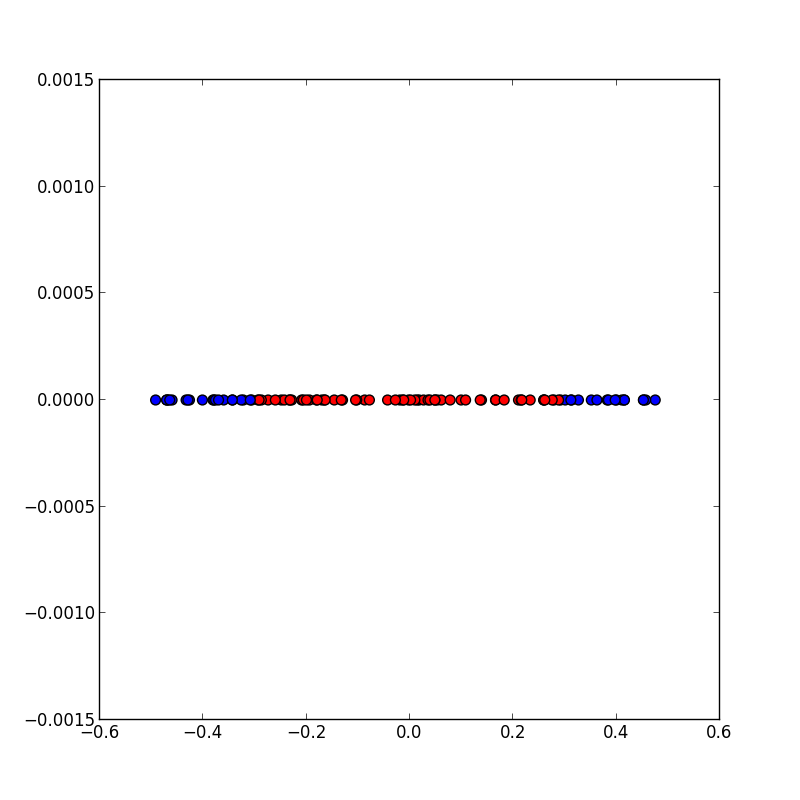
\includegraphics[scale=0.27]{images/pw1.png}
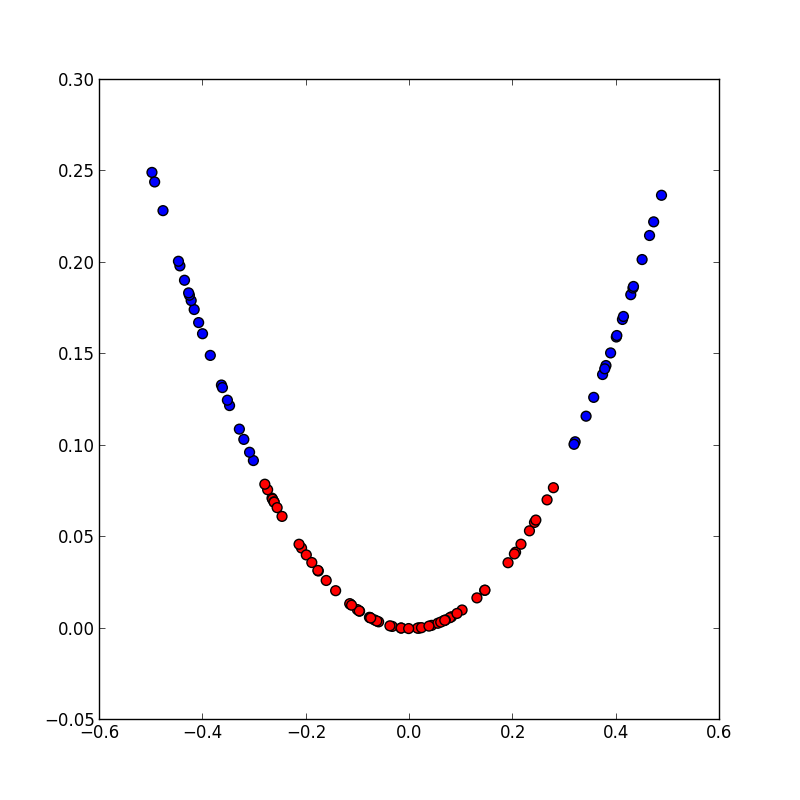
\includegraphics[scale=0.27]{images/pw2.png}
\end{center}

\end{frame}

\begin{frame}{Обобщенные линейные модели}

\begin{columns}[T]
    \begin{column}{.5\textwidth}
    Обучающая выборка
    
	$$X = (\mathbf{x}_1, \ldots, \mathbf{x}_N)$$
	
	Значения целевой переменной	
	
	$$t_1, \ldots, t_N; \quad t_j \in \{-1, +1\}$$
	    
    Функция принятия решения
    \[
    y(\mathbf{x}) = \mathbf{w}^\top \phi(\mathbf{x}) + b
    \]
    Разделяющая плоскость (РП)
    \[
    y_i(\mathbf{x_i}) t_i > 0
    \]
    Решений много: как выбрать?
    \end{column}
       
    \begin{column}{.5\textwidth}
    \vspace{-0em}
	\begin{center}
   		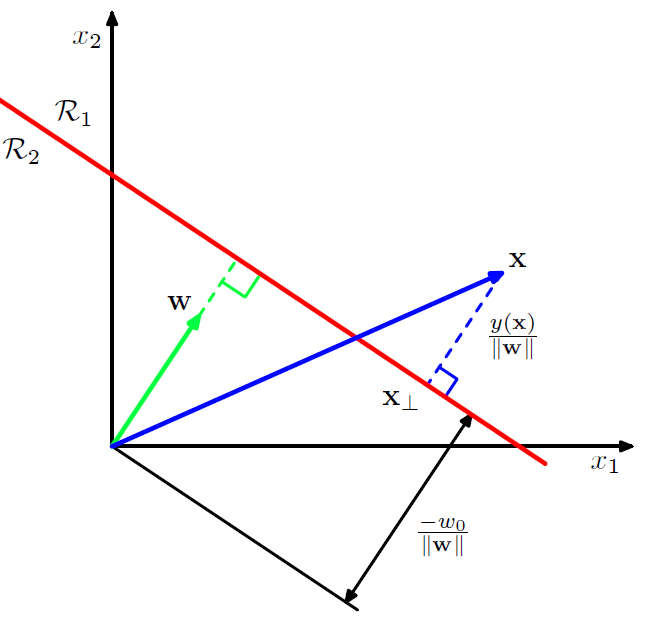
\includegraphics[scale=0.3]{images/linear.png}
    \end{center}
    \end{column}
  \end{columns}
  
\end{frame}

\begin{frame}{Максимальный зазор}

\begin{columns}[T]
    \begin{column}{.51\textwidth}
    Margin -- наименьшее расстояние между РП и обучающим объектом.
    \[
    d_j = \frac{|y(\mathbf{x}_j)|}{\|\mathbf{w}\|} = \frac{t_j y(\mathbf{x}_j)}{\|\mathbf{w}\|} = 
    \]    
    \[
    = \frac{t_j (\mathbf{w}^\top \phi(\mathbf{x}_j) + b)}{\|\mathbf{w}\|}
    \]
    Оптимальная РП
    \[
    \arg \max_{\mathbf{w}, b} \left[\frac{1}{\|\mathbf{w}\|} \min_j t_j (\mathbf{w}^\top \phi(\mathbf{x}_j) + b) \right]
    \]
	
    \end{column}
       
    \begin{column}{.5\textwidth}
    \vspace{-0em}
	\begin{center}
   		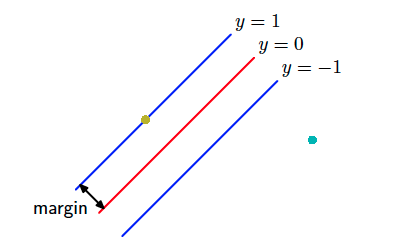
\includegraphics[scale=0.45]{images/margin.png}
    \end{center}
    \end{column}
  \end{columns}
  
\end{frame}

\begin{frame}{Задача оптимизации}

Расстояние от точки $x_j$ до РП
\[
d_j = \frac{t_j (\mathbf{w}^\top \phi(\mathbf{x}_j) + b)}{\|\mathbf{w}\|}
\]

Для точки $x_j$, лежащей на минимальном расстоянии от РП положим
\[
t_j (\mathbf{w}^\top \phi(\mathbf{x}_j) + b) = 1
\]

\begin{framed}
{\bf Задача оптимизации}
\begin{eqnarray*}
&& \frac 1 2 \|\mathbf{w}\|^2 \rightarrow \min_{\mathbf{w}, b} \\
&& \text{при условиях} \\
&& t_j (\mathbf{w}^\top \phi(\mathbf{x}_j) + b) \geq 1, \;\; \forall j \in 1,\ldots,N
\end{eqnarray*}
\end{framed}

\end{frame}

\begin{frame}{}

Метод множителей Лагранжа $\mathbf{a} = (a_1, \ldots, a_N)^\top,\;a_i \geq 0$.
\[
L(\mathbf{w}, b, \mathbf{a}) = \frac 1 2 \|\mathbf{w}\|^2 - \sum_{j=1}^N a_j [t_j (\mathbf{w}^\top \phi(\mathbf{x}_j) + b) - 1]
\]
Дифференцируем по $\mathbf{w}$ и $b$
\[
\mathbf{w} = \sum_{j=1}^N a_j t_j \phi(\mathbf{x}_j), \;\; 0 = \sum_{j=1}^N a_j t_j
\]
Подставляем $\mathbf{w}$ и $b$ в лагранжиан

\end{frame}

\begin{frame}{Сопряженная задача}

\begin{framed}
{\bf Сорпяженная задача}
\begin{eqnarray*}
&& \tilde{L}(\mathbf{a}) = \sum_{j=1}^N a_j - \frac{1}{2} \sum_{i=1}^N \sum_{j=1}^N a_i a_j t_i t_j \phi(\mathbf{x}_i)^\top \phi(\mathbf{x}_j) \rightarrow \max_{\mathbf{a}} \\
&& \text{при условиях} \\
&& a_j \geq 0, \;\; \forall j \in 1,\ldots,N \\
&& \sum_{j=1}^N a_j t_j = 0\\
\end{eqnarray*}
\end{framed}

Наблюдения
\begin{itemize}
\item $k(x_i, x_j) = \phi(\mathbf{x}_i)^\top \phi(\mathbf{x}_j)$ -- неотрицательно-определенная функция
\item лагранжиан $\tilde L(\mathbf{a})$ -- выпуклая и ограниченная сверху функция
\end{itemize}

\end{frame}

\begin{frame}{Классификация}

Функция принятия решения
\[
y(\mathbf{x}) = \mathbf{w}^\top \phi(\mathbf{x}) + b = \sum_{j=1}^N a_j t_j \phi(\mathbf{x}_j)^\top  \phi(\mathbf{x}) + b = \sum_{j=1}^N a_j t_j k(\mathbf{x}_j, \mathbf{x}) + b
\]
Условия Karush-Kuhn-Tucker
\begin{eqnarray*}
a_j &\geq& 0 \\
t_j y(\mathbf{x_j}) - 1 &\geq& 0 \\
a_j \{t_j y(\mathbf{x_j}) - 1\} &=& 0
\end{eqnarray*}
{\bf Опорным векторам} $\mathbf{x}_j \in S$ соответствуют $a_j > 0$
\[
b = \frac{1}{N_s} \sum_{i \in S} \left( t_i - \sum_{j \in S} a_j t_j k(\mathbf{x_i}, \mathbf{x_j})\right)
\]

\end{frame}

\begin{frame}{Линейно-разделимый случай}

\begin{block}{Задача}
Дана обучающая выборка

\begin{center}
\begin{tabular}{l|cc|c}
 & $x_1$ & $x_2$ & $t$ \\
 \hline
$\mathbf{x}_1$ & $1$ & $-2$ & $1$ \\
$\mathbf{x}_2$ & $1$ & $2$ & $-1$ \\
\end{tabular}
\end{center}

Найти оптимальную разделяющую плоскость, используя сопряженную задачу оптимизации

\end{block}

\end{frame}

\begin{frame}{Линейно-неразделимый случай}

\begin{center}
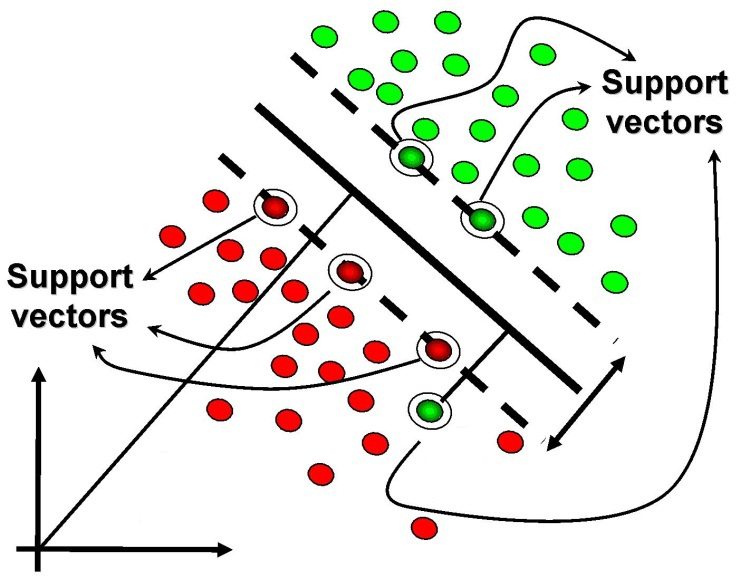
\includegraphics[scale=0.45]{images/svm.jpg}
\end{center}

\end{frame}

\begin{frame}{Смягчение ограничений}

\begin{columns}[T]
    \begin{column}{.51\textwidth}
    
    Переменные $\xi_j \geq 0$ (slacks):
    \[
    \xi_j = \begin{cases}
    0, \quad\quad\quad\quad\;\;\text{ если }y(\mathbf{x_j}) t_j \geq 1  \\
    |t_j - y(\mathbf{x}_j)|, \;\,\text{ иначе}
    \end{cases}
    \]
    Задача оптимизации
    \[
    C \sum_{j=1}^N \xi_j + \frac{1}{2}\|\mathbf{w}\|^2 \rightarrow \min_{\mathbf{w}, b}
    \]
    при условиях
    \[
		t_j y(\mathbf{x}_j) \geq 1 - \xi_j, \;\; \xi_j \geq 0
		\]

	
    \end{column}
       
    \begin{column}{.5\textwidth}
    	\vspace{-1em}
		\begin{center}
   			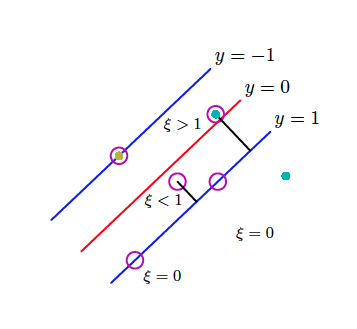
\includegraphics[scale=0.45]{images/slack.png}
    	\end{center}
	\end{column}
\end{columns}
  
\end{frame}

\begin{frame}{Сопряженная задача}

\begin{framed}
{\bf Сорпяженная задача}
\begin{eqnarray*}
&& \tilde{L}(\mathbf{a}) = \sum_{j=1}^N a_j - \frac{1}{2} \sum_{i=1}^N \sum_{j=1}^N a_i a_j t_i t_j \phi(\mathbf{x}_i)^\top \phi(\mathbf{x}_j) \rightarrow \max_{\mathbf{a}} \\
&& \text{при условиях} \\
&& 0 \leq a_j \leq C, \;\; \forall j \in 1,\ldots,N \\
&& \sum_{j=1}^N a_j t_j = 0\\
\end{eqnarray*}
\end{framed}

Наблюдения
\begin{itemize}
\item $a_j = 0$ -- правильно проклассифицированные объекты
\item $a_j = C$ -- опорные векторы внутри отступа 
\item $0 < a_j < C$ -- опорные векторы на границе
\end{itemize}

\end{frame}

\begin{frame}{Классификация}

Функция принятия решения
\[
y(\mathbf{x}) = \sum_{j=1}^N a_j t_j k(\mathbf{x}_j, \mathbf{x}) + b
\]
Константа $b$
\[
b = \frac{1}{N_\mathcal{M}} \sum_{i \in \mathcal{M}} \left( t_i - \sum_{j \in S} a_j t_j k(\mathbf{x_i}, \mathbf{x_j})\right)
\]

\end{frame}

\begin{frame}{Задача регрессии}

\begin{columns}[T]
    \begin{column}{.51\textwidth}
    
    Переменные $\xi_j \geq 0$, $\hat \xi_j \geq 0$ (slacks):
    \[
    t_j \leq y(\mathbf{x}_j) + \epsilon + \xi_n
    \]
     \[
    t_j \geq y(\mathbf{x}_j) - \epsilon - \hat \xi_n
    \]
    Задача оптимизации
    \[
    C \sum_{j=1}^N (\hat \xi_j + \xi_j) + \frac{1}{2}\|\mathbf{w}\|^2 \rightarrow \min_{\mathbf{w}, b}
    \]    
	
    \end{column}
       
    \begin{column}{.5\textwidth}
    	\vspace{0em}
		\begin{center}
   			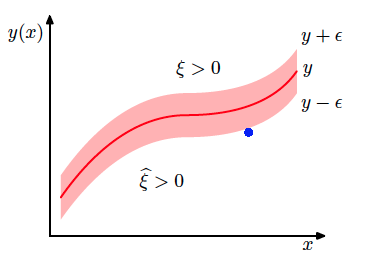
\includegraphics[scale=0.45]{images/regression.png}
    	\end{center}
	\end{column}
\end{columns}

\end{frame}

\begin{frame}{Численные методы оптимизации}

\begin{itemize}
\item Chunking (Vapnik, 1982)
\item Decomposition (Osuna, 1996)
\item Sequential Minimal Optimization (Platt, 1999)
\end{itemize}

\end{frame}

% ============================================== %

\section{Функции ядра}

% ============================================== %

\begin{frame}{}

\begin{center}
\Large Функции ядра
\end{center}

\end{frame}

\begin{frame}{Функции ядра}

$\phi(\mathbf{x})$ --  функция преобразования $\mathbf x$ из исходного пространства в спрямляющее пространство

\vspace{1em}
Проблема: количество признаков может быть очень велико

\vspace{1em}
\begin{block}{Идея Kernel Trick}
В процессе тренировки и применения SVM исходные векторы $\mathbf x$ используются только как аргументы в скалярном произведении $k(\mathbf x_i, \mathbf{x}_j) = \phi(\mathbf x_i)^\top \phi(\mathbf{x_j})$. Но в этом случае можно избежать вычисления $\varphi(\mathbf x)$!
\end{block}

\end{frame}

\begin{frame}{Теорема Мерсера}

\begin{alertblock}{Теорема}
Функция $k(\mathbf x, \mathbf z)$ является ядром тогда и только тогда, когда она 
\begin{itemize}
\item симметрична 
\[
k(\mathbf x, \mathbf z) = k(\mathbf z, \mathbf x)
\]
\item неотрицательно определена
\[
\int_{\mathbf x \in \mathbf X} \int_{\mathbf z \in \mathbf X} k(\mathbf x, \mathbf z) g(\mathbf x) g(\mathbf z) d\mathbf x d\mathbf z \geqslant 0, \;\; \forall g(\mathbf{x}): \mathbf{X} \rightarrow R
\]
\end{itemize}
\end{alertblock}

\begin{block}{Задача}
Пусть $\mathbf x \in R^2$, а преобразование $\phi(\mathbf{x})$
\[
\phi(\mathbf{x}) = (1, \sqrt{2} x_1, \sqrt{2} x_2, x_1^2, \sqrt{2} x_1 x_2, x_2^2).
\]
Проверить, что функция $k(\mathbf{x}, \mathbf{z}) = (1 + \mathbf x^\top \mathbf z)^2$ является функцией ядра для данного преобразования.
\end{block}

\end{frame}

\begin{frame}{Некоторые стандартные функции ядра}

\begin{itemize}
\item Линейное ядро
\[
k(\mathbf{x}, \mathbf{z}) = \mathbf{x}^\top\mathbf{z}
\]
\item Полиномиальное ядро степени $d$
\[
k(\mathbf{x}, \mathbf{z}) = (\mathbf{x}^\top\mathbf{z} + r)^d
\]
\item Radial Basis Function
\[
k(\mathbf{x}, \mathbf{z}) = e^{-\gamma |\mathbf x - \mathbf z|^2}
\]
\item Sigmoid
\[
k(\mathbf{x}, \mathbf{z}) = \tanh (\gamma \mathbf{x}^\top\mathbf{z} + r)
\]

\end{itemize}

\end{frame}

\begin{frame}{Опять ирисы}

\begin{center}
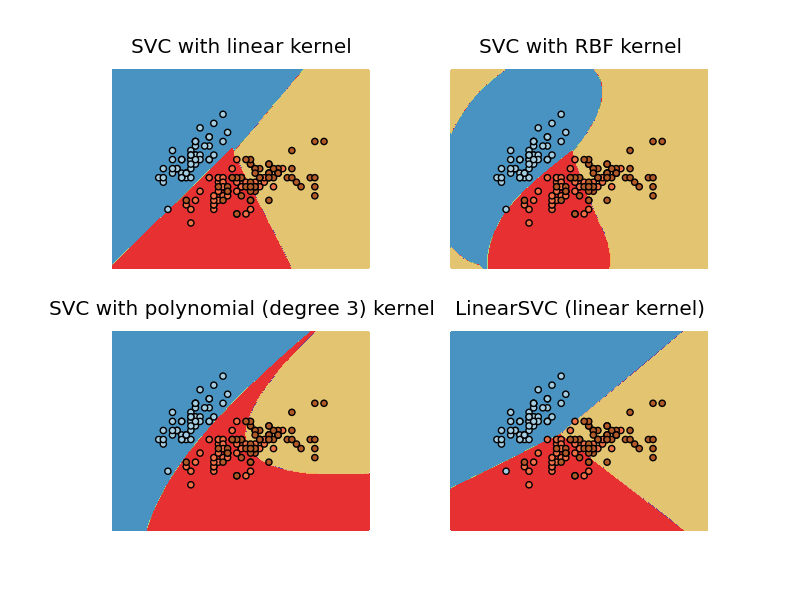
\includegraphics[scale=0.5]{images/iris.png}
\end{center}

\end{frame}

% ============================================== %

\section{SGD}

% ============================================== %

\begin{frame}{}

\begin{center}
\Large SGD
\end{center}

\end{frame}

\begin{frame}{Связь с линейными моделями}

Задача оптимизации 
\[
C \sum_{j=1}^N \xi_j + \frac{1}{2} \|w\|^2 \sim \sum_{j=1}^N E(y(\mathbf{x}_j), t_j) + \lambda \|w\|^2 \rightarrow \min_{\mathbf{w}, b}
\]
Hinge loss
\[
E(y_j, t_j) = \begin{cases}
1 - y_j t_j, \text{ если } y_j t_j < 1 \\
0, \quad\quad\;\;\,\text{ иначе }
\end{cases}
\]

\end{frame}

\begin{frame}{Stochastic Gradient Descent}

Градиентный спуск
\[
\mathbf{w}_{k+1} = \mathbf{w}_k - \eta(k) \frac 1 N \sum_{n=1}^N \nabla_\mathbf{w} l(\mathbf{x_n, \mathbf{w}}, t_n)
\]
Стохастический градиентный спуск
\[
\mathbf{w}_{k+1} = \mathbf{w}_k - \eta(k) \nabla_\mathbf{w} l(\mathbf{x_k, \mathbf{w}}, t_k)
\]
Усредненный стохастический градиентный спуск $\bar{\mathbf{w}}_k = \frac 1 k \sum_{j=1}^k \mathbf{w}_j$
\[
\mathbf{w}_{k+1} = \mathbf{w}_k - \eta(k) \nabla_\mathbf{w} l(\mathbf{x_k, \mathbf{w}}, t_k), \quad \bar{\mathbf{w}}_{k+1} = \frac{k}{k+1} \bar{\mathbf{w}}_{k} + \frac{1}{k+1} \mathbf{w}_{k+1}
\]
Сходимость: $\sum_k \eta_k^2 < \infty, \;\; \sum_k \eta_k = \infty$

\end{frame}

\begin{frame}{SGD tips}

\begin{itemize}
\item Использовать SGD, когда обучение модели занимает слишком много времени
\item Перемешать тренировочную выборку
\item Следить за training error и {\bf validation error}
\item Поверять, правильно ли вычисляется градиент 
\[
Q(z, w + \delta) \approx Q(z, w) + \delta g
\]
\item Подобрать $\eta_0$ на небольшой выборке 
\[
\eta_k = \eta_0 (1 + \eta_0 \lambda k)^{-1}, \quad \lambda\text{ -- параметр регуляризации}
\] 
\end{itemize}

\end{frame}

\begin{frame}{SVM -- итоги}

\begin{itemize}
\item[+] Нелинейная разделяющая поверхность
\item[+] Глобальая оптимизация
\item[+] Разреженное решение
\item[+] Хорошая обобщающая способность
\item[-] Не поддерживает $p(C_k | \mathbf x)$
\item[-] Чувствительность к выбросам
\item[-] Нет алгоритма выбора ядра
\item[-] Медленное обучение
\end{itemize}

\end{frame}

\begin{frame}{}

\begin{center}
\Large Вопросы
\end{center}

\end{frame}

\end{document}